
\documentclass{article}
\title{Sailor GSoC Report}
\date{May 25th 2015}
\author{Etiene Dalcol}
\usepackage{listings}   
\usepackage{hyperref}
\usepackage[T1]{fontenc}
\usepackage[backend=bibtex,style=verbose-trad2]{biblatex}
\usepackage{graphicx}
\usepackage[a4paper, total={6in, 8in}]{geometry}       
\bibliography{main} 
\begin{document}
	\pagenumbering{gobble}

\begin{titlepage}

\newcommand{\HRule}{\rule{\linewidth}{0.5mm}} % Defines a new command for the horizontal lines, change thickness here

\center % Center everything on the page
 
%----------------------------------------------------------------------------------------
%	HEADING SECTIONS
%----------------------------------------------------------------------------------------

\textsc{\LARGE École Nationale Supérieure de Techniques Avancées Bretagne}\\[0.5cm] % Name of your university/college

\includegraphics[scale=0.15]{enstalogo.jpg}\\[0.5cm]
\textsc{\Large Summer Internship Report}\\[0.5cm] % Major heading such as course name
\textsc{\large Web development in Lua programming language}\\[0.5cm] % Minor heading such as course title

%----------------------------------------------------------------------------------------
%	TITLE SECTION
%----------------------------------------------------------------------------------------

\HRule \\[0.4cm]
{ \huge \bfseries Improvements to Sailor framework during Google Summer of Code}\\[0.4cm] % Title of your document
\HRule \\[0.5cm]



\includegraphics[scale=0.15]{logo-lua.png}

\includegraphics[scale=0.3]{gsoclogo.jpg}\\[1.5cm]
 
%----------------------------------------------------------------------------------------
%	AUTHOR SECTION
%----------------------------------------------------------------------------------------

\begin{minipage}{0.4\textwidth}
\begin{flushleft} \large
\emph{Author:}\\
Etiene \textsc{da Cruz Dalcol} % Your name
\end{flushleft}
\end{minipage}
~
\begin{minipage}{0.4\textwidth}
\begin{flushright} \large
\emph{Supervisor:} \\
Dr. Olivier \textsc{Reynet} % Supervisor's Name
\end{flushright}
\end{minipage}\\[1.5cm]

% If you don't want a supervisor, uncomment the two lines below and remove the section above
%\Large \emph{Author:}\\
%John \textsc{Smith}\\[3cm] % Your name

%----------------------------------------------------------------------------------------
%	DATE SECTION
%----------------------------------------------------------------------------------------

{\large \today}\\[3cm] % Date, change the \today to a set date if you want to be precise

%----------------------------------------------------------------------------------------
%	LOGO SECTION
%----------------------------------------------------------------------------------------


% Include a department/university logo - this will require the graphicx package


 
%----------------------------------------------------------------------------------------

\vfill % Fill the rest of the page with whitespace

\end{titlepage}




	\newpage
	\tableofcontents

	\newpage
	\pagenumbering{arabic}

	\section{Abstract}

Lua is a very fast and powerful scripting language that can be easily embeddable. For that reason, it has gained a niche in the game development industry. Lua has great potential and incredible benchmarks. Despite being also an excellent tool as a general purpose language to develop robust applications, its use in web developments needs to be more widespread. \\

Sailor was invented to increase the ecosystem of web development in Lua but it is still in early development. The purpose of this work is to turn Sailor into a more mature software by adding new features and improving existing ones such as adding automated tests and improving the use of Lua instead of Javascript when programming for the browser. 

	\subsection*{Resumé}\\
Lua est un langage très rapide et puissant qui peut être embarqué facilement. Pour cette raison, il a gagné une place importante dans l'industrie de développement de jeux. Lua a des potentiels et benchmarks incroyables. En dépit d'être aussi un excellent outil en tant que langue d'usage général pour développer des applications robustes, son utilisation dans le développement web devrait être plus généralisée.\\

Sailor a été inventé pour augmenter l'écosystème du développement web en Lua, mais il est encore dans un stage de développement précoce. Le but de ce travail est de transformer Sailor dans un logiciel plus mature en ajoutant de nouvelles fonctionnalités et l'amélioration de ceux existants, tels que l'ajout de tests automatisés et d'amélioration de l'utilisation de Lua lieu de Javascript lors de la programmation pour le navigateur.


	\newpage
	
	\section{Introduction}

	\subsection{Google Summer of Code}
	Google Summer of Code (GSoC) is a global program that connects students with open source, free software and technology-related organizations. During the a 3 month period on the summer, the students get familiarised with open source projects, work with the community and write code. \\

Google identifies open source projects and organizations that will receive funding and participate on the program. The organizations will provide mentors to guide students during the program. Students submit projects to the organizations, who rank them. Organizations may suggest a list of ideas for projects. Once Google defines how many student slots for projects are allocated to an organization, the organization decides which students and projects are accepted and pair them with a mentor.\\

While most students come from a Computer Science and Software Engineering background, this is not mandatory and the educational area of participants can be very wide.\\

The program is centered on some goals\autocite{gsocgoals}:
\begin{quote}\begin{enumerate}\item Get more open source code written and released for the benefit of all.
\item Inspire young developers to begin participating in open source development.
\item Help open source projects identify and bring in new developers.
\item Provide students the opportunity to do work related to their academic pursuits during the summer: "flip bits, not burgers."
\item Give students more exposure to real-world software development (for example, distributed development and version control, software licensing issues, and mailing list etiquette)."
	\end{enumerate}
\end{quote}

There are midterm and final evaluations, and the code completed must be submitted to GSoC's website by the end of the program. All development happens online, Google does not provide an office space and there's no requirement to travel.\\

Since the start of the program, in 2005, over 8500 successful students have participated, from over 109 countries, with 8000 mentors making 55 million lines of code.


\subsection{LabLua}
	
LabLua was one of the organizations selected to participate in the 2015 version of Google Summer of Code. It is a research lab at the Pontifical Catholic University of Rio de Janeiro (PUC-Rio) affiliated with its Computer Science Department. Its researches are on the field of programming languages, with an emphasis on the Lua programming language. The founder of LabLua, Prof. Roberto Ierusalimschy, is one of the creators of the Lua language.\\

LabLua proposed the following list of ideas to GSoC: 

\begin{enumerate}\item LuaRocks add-ons system
\item Port Lua Test Suite to NetBSD Kernel
\item Elasticsearch Lua client (elasticsearch-lua)
\item Add support for left recursion to LPeg
\item Switch Typed Lua from optional typing to gradual typing
\item Adapt CGILua SAPI launcher to explore all WSAPI features
\item Add support for WSDL generation to LuaSOAP
\item Add support for prepared statements in LuaSQL
\item Multi-CPU usage in VLC
\item Multi-CPU usage in wireshark
\item Develop a binary serialization format with support for dynamically types values and an RPC protocol for dynamically typed invocations based on this format.
\item Develop a library for Lua that allows Lua programs to access features provided by the platform's underlying operating system (OS) kernel, such as process control, network access, file system, event notification, etc.
\item Port an SDL-based C++ open source game to Céu
\end{enumerate}

They received in total 6 slots, from which, four of them were filled by students working on ideas 2, 3, 7 and 13 and two of them were ideas proposed by students themselves. One of the student-proposed ideas was my project to improve Sailor, a web development framework I had been developing on my free time. \\

The project was mentored by Dr. Fabio Mascarenhas, professor at Universidade Federal do Rio de Janeiro. Since Google did not provide for office space or work placement, ENSTA Bretagne offered a placement during the summer to work on this project under the supervision of Professor Dr. Olivier Reynet. \\

\subsection{The Lua programming language}

\begin{quotation}Lua is a powerful, fast, lightweight, embeddable scripting language.\autocite{luaorg}\end{quotation}

This description provided by lua.org does not fully grasp what's interesting about this language. Lua was created in a very specific context: Petrobras, a multinational energy and oil corporation headquartered in Rio de Janeiro, Brazil had interactive graphical programs for engineering applications. These programs needed some flexibility and they were used by non professional programmers. Lua was created to be very simple yet powerful, allowing the customisation of these softwares through scripting. Avoiding cryptic syntax and semantics, Lua is a very readable language with a short learning curve. \\

It's possible to have an idea about the simplicity of this language just by comparing the brevity of the Programming in Lua book versus books on pretty much any other language. This means you can have all of the language in your head. Its source code is also very succinct. As of version 5.3.1, described in about 23000 lines of Standard C, the whole distribution which includes documentation has only 276Kb. This allows easily porting Lua code to things that run standard ANSI C, even if they have typically low resources, and embedding Lua to applications without bloating them. The result is that Lua is a very widely used language, from micro controllers and washing machines to operating systems, power computers and video games.\\

Its power can be observed on its multi-paradigm extensible semantics and speed. For example, while Lua does not come with Object Oriented Programming out of the box, it is possible to prototype it using first class functions \footnote{Support of passing functions as arguments to other functions, returning them as the values from other functions, and assigning them to variables or storing them in data structures. \autocite{wikifunc}} and metatables \footnote{Allows to change the behavior of a table. It is part of an extension mechanism which allows you to overload certain operations on Lua objects. \autocite{luausersmeta} \autocite[117]{pil}}. Lua also performs way better than other popular programming languages on speed tests. A special dialect of Lua called LuaJIT is the fastest it can get while still being a dynamically typed scripting language\autocite[8]{modlua}: \\

%\clearpage
\begin{figure}[h]
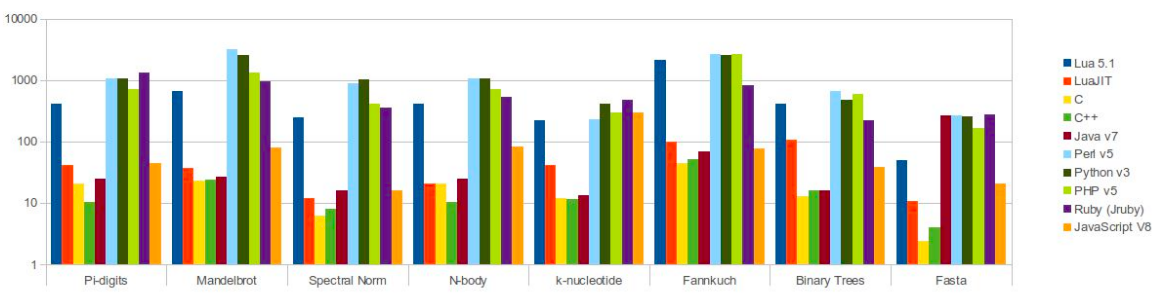
\includegraphics[scale=0.4]{speed.png}
\caption{\label{fig:speedcomparison} Speed comparison of popular script languages (less is better)}
\end{figure}

	\newpage
\section{Analysis of the problem}

Lua is greatly used as an embedded language and has found a niche in game development being the top language of choice for scripting in this area\autocite{engine}. In the same time, it is still a great tool as a general purpose language but not much widespread in other domains such as web development. As of September 26th of 2015 Lua is used in less than 0.1\% of websites whose server-side programming language we know\autocite{w3server}. \\

\begin{figure}[h]
\centering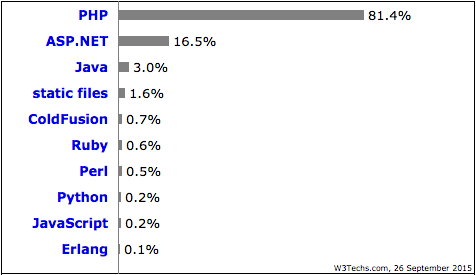
\includegraphics[scale=0.7]{serverlangs.png}
\caption{\label{fig:serverlangs} Usage of server-side programming languages for websites. Note: a website may use more than one server-side programming language}
\end{figure}

In an attempt to understand why this happens, I made an analysis of the context of the top used language: PHP. One may argue that PHP is not such a well-designed language. Then why is it the top language of choice for web development? Why is 82\% of the web made of PHP websites? We could speculate that PHP's success is due to a good timing but, 20 years later, allegedly better programming languages have appeared and PHP's popularity continues to grow\autocite{phptime}.\\

\clearpage
\begin{figure}[h]
\centering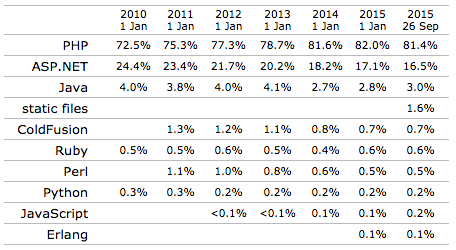
\includegraphics[scale=0.7]{serverlangstime.png}
\caption{\label{fig:serverlangstime} Historical yearly trends in the usage of server-side programming languages for websites}
\end{figure}


This is what Jeff Atwood, stackoverflow co-founder, calls "The PHP singularity"\autocite{phpsing}. According to him, the faults of PHP don't matter because it has a huge ecosystem and easy deployment and the only solution to this is to build compelling alternatives who are as pervasive and as easy to setup and use. In his blog, he calls out the community of programmers to push other options forward.\\

Having some knowledge of the PHP ecosystem as a beginner and intermediate user, I considered this an interesting challenge. As Lua is a well-designed, fast and easy-to-learn language, I believe it is a perfect candidate for the job in terms of quality. But how about it's ecosystem?\\

\subsection{The Lua ecosystem}

\subsubsection{General ecosystem}

Despite being a successful 20-year old language, Lua's community and amount of libraries is small. This is an issue that is being addressed, specially in the recent years. The Kepler Project\autocite{kepler} (2006-2009) was a project developed with the goal to make a platform for web development in Lua\autocite{cgilua}. While it did not accomplish its ultimate goal, it produced some of the modules that were essential for the later development of the ecosystem. One of these modules that deserves a highlight is LuaRocks\autocite{luarocks}, developed by Hisham Muhammad to deploy Kepler modules. LuaRocks is now the package manager for Lua modules, acting as a one-stop repository that significantly reduced the entry barrier for Lua as an application development language. Pierre Chapuis, in his 2013 talk "State of the Lua Ecosystem"\autocite{luaeco} suggested modules should be even easier to find. He created a website called Lua toolbox\autocite{luatoolbox}, aimed at ranking, endorsing and classification of Lua modules. In the meantime, MoonRocks, a tool aimed at easy uploading and hosting of modules\autocite{moonrocks} was created by Leaf Corcoran, also in 2013. This project has recently merged with LuaRocks. \\

All these efforts have been producing results and the ecosystem is growing steadily\autocite{luarockspresentation}: \\
\begin{figure}[h]
\centering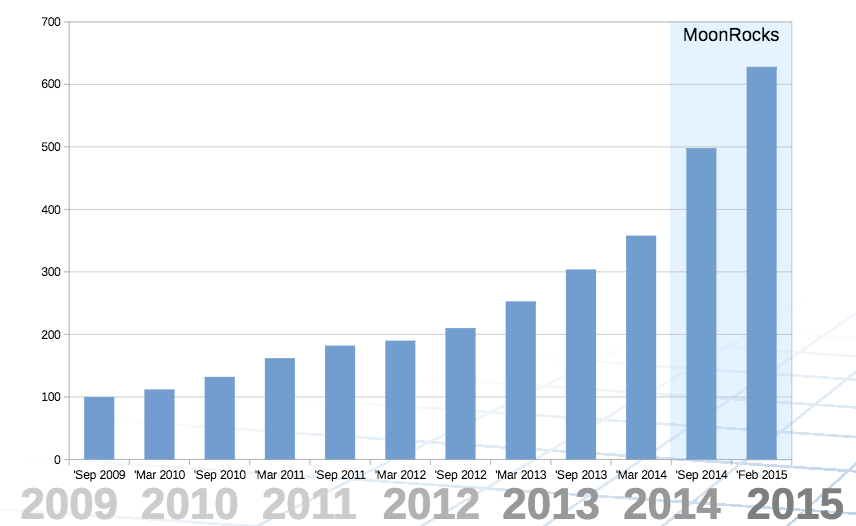
\includegraphics[scale=0.5]{luamodules.png}
\caption{\label{fig:luamodules} Recent growth of the repository}
\end{figure}

\subsubsection{Web servers supported}

Lua can run on a variety of web servers. Apache has a module to run lua called mod\_lua, Nginx has a distribution called open resty that allows to run Lua too. This is great news, because they are the top two web servers used\autocite{webservers}. There’s Xavante, which is a web server written in Lua and allows a really quick deploy, as well as plenty of others options like Mongoose, Lwan or Lighttpd. 
\begin{figure}[h]
\centering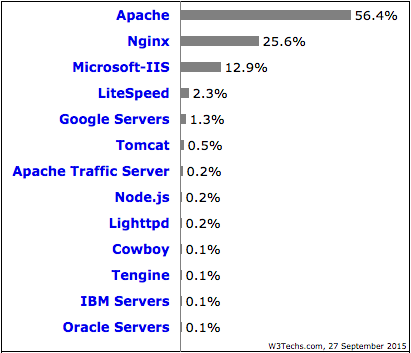
\includegraphics[scale=0.7]{webservers.png}
\caption{\label{fig:webservers} Usage of web servers for websites}
\end{figure}

\subsubsection{Existing tools and frameworks}

\textbf{Orbit:} \\

Orbit is the longest established framework the Lua community has, but it's not in active development anymore. It's very lightweight and follows an MVC architecture. \\

Can be installed through LuaRocks: Yes\\

Documentation: Very succinct but sufficient\\

License: GPL\\

Website: \url{http://keplerproject.github.io/orbit/}\\

\textbf{Luvit:}\\

Luvit adopts a different kind of approach from Orbit. It's designed to be a port of Node.js to Lua. It accomplishes this task very well, claiming to be 2 to 4 times more performant and making great memory savings. However, for those that are not already proficient in writing applications with Node.js, it can be very complex to use as its documentation is not yet prepared to receive full beginners in the web development world. It's very powerful, it's in intense development and it is maybe the most popular Lua web development framework, but still very little known outside the community.\\

Can be installed through LuaRocks: No\\

Documentation: Insufficient\\

License: Apache 2.0\\ 

Website: \url{https://luvit.io/}\\ 

\textbf{Lapis:}\\

Lapis is a very interesting framework. It's not exactly in Lua, but in MoonScript, a language that compiles to Lua like CoffeeScript compiles to JavaScript. You can still, however, use Lua to write your application. It's in very active development by a dedicated maintainer. It does not provide an MVC architecture out of the box but it's possible to prototype one. \\

Can be installed through LuaRocks: Yes\\ 

Documentation: Extensive and informative\\

License: MIT\\

Website: \url{http://leafo.net/lapis/}\\

\textbf{Other projects worth mentioning:}\\

TurboLua | Apache 2.0: \url{http://www.turbolua.org/} \\

Tir | BSD: \url{http://tir.mongrel2.org/} \\

Ophal | AGPL 3.0: \url{http://ophal.org/} \\

	\newpage
\section{Proposal}

As seen at the ecosystem analysis, while Lua already provides a set of libraries and tools for web development, none of them has reached a somewhat wide-spread use in the web development community. And while the Lua ecosystem seems to be flourishing nicely, this set is still considerably small comparing to the amount of tools offered in other programming languages. Having this in mind, I considered that building a new tool for web development in Lua was not a redundant task. As a follow-up to Atwood's call for action, I decided to push and advocate Lua as a promising platform and simply create more options. In the worst-case scenario I would learn a lot of things about the Lua programming language and about web development. \\

This idea was the beginning of Sailor, a framework for fast development of web applications in Lua I started developing in 2014. In the same way as Lua, Sailor is free software and written under the MIT License. Its applications are structured in a model-view-controller (MVC) architecture. Like other web development frameworks, such as Ruby on Rails, it is designed to make the development process faster by making some assumptions and conventions (not requiring configuration for everything) and encouraging principles like DRY (Don't Repeat Yourself).\\

Its ultimate goal is to be very easy to use while still being a high quality tool. Sailor offers many possibilities of setup to its users, can be used for building projects of any size in such a friendly language that is Lua and allows the use of Lua in the client-side (browser) as well, eliminating the use of JavaScript if desired.\\

This last point is a really interesting aspect of this project. Writing code in Lua to run in the browser is allowed through an integration of Sailor with a Lua-to-Javascript virtual machine. While it will be less performant, there are other advantages. Usually, a beginner web developer needs to learn at least 4 types of languages for building a complete dynamic website, including those that are not considered programming languages: a server side language of choice, JavaScript for the client side, HTML / CSS and SQL. Being able to use the same language for both the server and the client side reduces the entry barrier and improves maintainability and reusability of the code. In addition to this, with the beginning of the development of Web Assembly\autocite{webassembly} in April 2015, the possibility to run Lua natively on browsers may be attained in the foreseeable future, which is very promising.\\


\textbf{Sailor Characteristics as of version 0.3 - Jupiter}\\

Features: Routing, ORM, Validation, Themes and Layouts, Bootstrap integration, Sessions, Cookies, friendly URLs, auto generator of models and CRUDs, easy form module, Lua in the browser, LuaRocks setup\\

Lua version compatibility: 5.1 and 5.2\\

Operating Systems: Windows, Mac or Linux\\

Web servers: Apache with mod\_lua, OpenResty distribution of Nginx, Xavante, Lwan ou Lighttpd.\\

Databases: MySQL, PostgreSQL, SQLite and other databases supported by the LuaSQL library.\\

Lua-to-JS virtual machine: Lua5.1.js (a 5.1 coding style is required for the client side)\\

Dependencies:
\begin{enumerate}\item lua >= 5.1, < 5.3
\item datafile >= 0.1
\item luafilesystem >= 1.6.2
\item valua >= 0.2.2
\item lbase64 >= 20120807
\item cgilua >= 5.1.4, < 5.2
\item xavante >= 2.3
\item wsapi-xavante >= 1.6.1 
\end{enumerate}\\

Licence: MIT\\

Website: \url{http://sailorproject.org}\\

\subsection{The Summer Project Proposal}

Sailor is a work in progress with a small codebase that is growing gradually. The project submitted to Google Summer of Code was focused on developing a new feature and improving an existing one: \\

\begin{enumerate}\item Implementing a test suite
\item Improving the usability of Lua at the client side
\end{enumerate}\item \\

The results would significantly increase the overall quality and usability of Sailor. In addition, Sailor's participation in GSoC could allow it to get more traction, which would be beneficial for both Sailor and the Lua community as it introduces some fresh blood into the current Lua web development scene. 

\subsection{Proposed development schedule}

		\begin{description}
	  \item[May 25th - June 5th] \hfill \\
	  Researching how other frameworks use their test suites
	  \item[June 6th - June 15th] \hfill \\
	  Researching and testing existent test Lua modules
	  \item[June 16th - July 1st] \hfill \\
	  Either integrating an existing test module with Sailor or developing a new one
	  \item[July 2nd - July 16th] \hfill \\
	  Testing, bug fixing and documenting
			\item[July 17th - July 23rd] \hfill \\
	  Researching and testing Lua to JavaScript VMs. E.g. MoonshineJS
			\item[July 24th - August 6th] \hfill \\
	  Improving current way to manipulate DOM from Lua and load Lua modules to be used on client side.
			\item[August 7th - August 16th] \hfill \\
	  Testing, bug fixing and documenting
			\item[August 17th - August 21st] \hfill \\
	  Polishing and making sure nothing was missed
		\end{description}
		
\newpage
\section{The development}

\subsection{Implementing a test suite}

Testing is a crucial part of software development. It is so important that there are development techniques that focus on that, such as Test-driven development (TDD). In TDD, first, an initially failing test for a function is written, and then a function that passes the test is developed. \\

Writing tests is useful not only for assuring that the software does what it is meant to do, but also that it will still do what its meant in different environments, with different inputs, within a reasonable time. By writing automated tests, there's a documentation of which cases the software is being tested against and the tests can be rerun when changes are made to the software or the environment to ensure that the expected results are still obtained.\\

As of version 0.3 Jupiter, Sailor did not provide an easy functionality to write automated tests to its applications.\\

The first step about implementing a test suite into Sailor was to investigate how this is done on different frameworks. A number of frameworks presented a functionality to test the applications made with them and insightful documentation such as Yii (PHP)\autocite{yiiguide} , Laravel (PHP)\autocite{laravel} , Lapis (Lua)\autocite{lapis} , Ruby on Rails (Ruby)\autocite{rails}  and Flask (Python)\autocite{flask} .\\

It was observed that the most common forms of application testing in web development had:\\

\begin{enumerate}
\item Fixtures: the ability to load sample data into a test database
\item Unit tests: the ability to test very specific pieces of code such as model methods
\item Functional tests, also called integration tests: the ability to test broader pieces of code and how they work together in the flux of the application use, such as the execution of a controller action
\end{enumerate}\\

There was little to no variation in how unit tests were done but what was defined as their functional tests varied a lot. Some frameworks mocked up a request, some frameworks launched a test server and made actual HTTP requests. Some frameworks provided even more complex testing, in a third category, for deeply testing the interface and included, for example, the simulation of mouse clicks in a web page. \\

For the purpose of this project, it was decided that mocking a request and executing Sailor's internal functions for running controller actions would be enough.\\

Investigating if there were already libraries that provided tests in Lua was not difficult. There aren't many around. Busted\autocite{busted}  is one of the top Lua libraries used with this purpose, it is in active development and well maintained, so it seemed like an obvious choice. \\

Before starting the integration of Sailor with Busted, some modifications to Sailor were necessary:\\

\begin{enumerate}\item Multiple databases\\
As of version 0.3, Sailor allowed the configuration of a database to be used by the application. This was changed to allow defining multiple database configurations and change environments to facilitate changing databases for testing.

\item Validation toggle \\
Normally, before saving a model, its attributes were validated. Now it is possible to turn off the validation if desired. This is useful for loading fixtures into the test database regardless if they are following the normal validation rules or not since testing with faulty inputs might be desired.
model:save() -> model:save(validate)
the default is true

\item Adding count method to model \\
This modification was not strictly necessary since the counting of entries in a table could be done manually, but this would facilitate making assertions and reduce the amount of code written for tests.

\item Renaming and restructuring Sailor's binary\\
When Sailor was installed, it installed a binary called sailor\_create, useful for rapidly creating new blank applications. Now that it would gain a new utility, it was renamed to simply sailor, being able to receive two commands: create and test.
\end{enumerate}

\lstset{language=Bash}    
\begin{lstlisting}[frame=single]
sailor create "My Application"
cd my_application
sailor test
\end{lstlisting}


\subsubsection{Busted integration}

A new module was added to Sailor, called tests. As of now it contains two important functions:

\lstset{language=Lua}    
\begin{lstlisting}[frame=single]
test.request(path, data, additional_headers)
\end{lstlisting}

Makes a mockup request to a certain path of a Sailor application.

\begin{description}\item \textbf{path}: \textit{string}. The path you want to make a request to, such as a controller or controller/action. Example: 'user/view'
\item \textbf{data}: \textit{table}. A table containing some data you want to send to the request, such as get or post. Example: {get = {id = 1}}
\item \textbf{additional\_headers}: \textit{table}. A table containing additional headers you may want to send. Example: {ACCEPT = 'application/json'}
\end{description}\\

This function will return a result table with the following fields:\\
\begin{description}\item \textbf{res.status}: \textit{number}. The status of the response.
\item \textbf{res.body}: \textit{string}. The body of the response.
\item \textbf{res.headers}: \textit{table}. Any headers out that were set.
\item \textbf{res:redirected(path)}: \textit{function}. A function that receives an internal Sailor app path and sees if the request was redirected there.\\
\end{description}\\

\begin{lstlisting}[frame=single]
test.load_fixtures(model_name)
\end{lstlisting}
Loads tests fixtures into the database.\\
\textbf{model\_name}: \textit{string}. The name of the model to be loaded.\\
Returns a table with the objects created.\\

A new function was also added to the form module.
\begin{lstlisting}[frame=single]
form.ify(object)
\end{lstlisting}
\textbf{object}: Sailor model object.\\
Returns a table of attributes of this model as they would be if sent via POST through a Sailor form. This is useful for mocking a POST request.  \\

Sailor applications now will come with a new directory called tests. It is organised in the following structure:\\

\begin{lstlisting}[frame=single]
fixtures/
unit/
functional/
bootstrap.lua
helper.lua
\end{lstlisting}\\\\

The fixtures/ directory will contain the fixture files. In Sailor, they are Lua files with the same name as the respective models that they are testing. They must return a table with the sample data. It is important to note that loading the fixtures will truncate existing data so it is important to configure the separate database for running tests on /conf/conf.lua.\\

Example fixture for testing an User model with two attributes, username and password:\\

\begin{lstlisting}[frame=single]
-- /tests/fixtures/user.lua

return {
    {
        username = 'joao',
        password = '123456'
    },

    {
        username = 'maria',
        password = '1234'
    }
}
\end{lstlisting}\\\\

The bootstrap.lua file contains code that the user may wish to be executed before running their tests. It is useful, for example, to load the fixtures:\\

\begin{lstlisting}[frame=single]
--/tests/bootstrap.lua
...
local t = require "sailor.test"
t.load_fixtures('user') 
\end{lstlisting}\\\\

The helper.lua file should be used to write functions that will be shared among different tests, like a helper library.\\

The unit/ directory will contain the unit tests files. The test scripts must follow a format specified by Busted. More features and details can be found at Busted’s website. A basic flow includes calling a describe function passing a description and a callback function that calls one or more it functions tests, also with a description and a callback containing specific tests and assertions. A very simple test could be written as follow:\\

\begin{lstlisting}[frame=single]
 -- /tests/unit/user_test.lua 
describe("Testing User model", function()
    local User = sailor.model('user')
    local fixtures = require "tests.fixtures.user"     

    it("should create a new user", function()
        local count_before = User:count() 
        -- Counting current users
        local u = User:new(fixtures[1])   
        -- Creating one more user with one of the fixtures
        assert.is_true(u:save(false))    
        -- Asserting that it saves
        assert.is_equal(User:count(),count_before+1)
        -- Asserting that the count increases by one
    end)
    -- ... more tests
end)
\end{lstlisting}\\\\

The functional/ directory contains functional tests. They must follow the same format specified by Busted as the unit tests. Here is an example of a functional test script, containing two tests and four assertions, using Sailor:\\

\begin{lstlisting}[frame=single]
-- /tests/functional/user_controller_test.lua 
describe("Testing User Controller", function()
    local User = sailor.model('user')
    local test = require "sailor.test"
    local form = require "sailor.form"
    local fixtures = require "tests.fixtures.user"

    it("should open index", function()
        local res = test.request('user/index') 
        -- Getting the response a mock request to 
        --  the index of the controller
        assert.same(200,res.status)       
        -- Asserting that the status of the response is ok
        assert.truthy(res.body:match('View all'))  
        -- Asserting that the page contains a string 'View all'
    end)

    it("should create a new user", function()
        local count_before = User:count()    
        -- Counting current users
        local res = test.request(
        	  'user/create', 
        	  {post = form.ify(fixtures[1])}
        	) 
        -- Posting some user to the 'user/create' page of your app
        assert.same(Category:count(), count_before + 1)   
        -- Asserting that the number of users increased by 1
        assert.is_true(res:redirected('user/index'))  
        -- Asserting that the page redirected you to the index
    end)
end)
\end{lstlisting}\\

\subsubsection{Running tests}

To run tests all that's needed to be done is to go to the app's directory and type sailor test or sailor t on command line. It is also possible to pass some flags that are accepted by Busted.\\

Example:
\begin{lstlisting}[frame=single]
cd my_app
sailor test --verbose
\end{lstlisting}\\

There should be an output like this:
\begin{lstlisting}[frame=single]
************************
24 successes / 0 failures / 0 errors / 0 pending : 0.04076 seconds
\end{lstlisting}






	\newpage

%\printbibliography
%\printbibheading[title={References},heading=bibnumbered]
\section{References}
	\printbibliography[title={Books},type=book,heading=subbibnumbered]
	\printbibliography[title={Articles},type=article,heading=subbibnumbered]
	\printbibliography[title={Websites},type=misc,heading=subbibnumbered]

	\newpage
	\section{Appendix}
	\begin{appendix}
	%\addcontentsline{toc}{subsection}{List of Figures}
	 \listoffigures
	 % \addcontentsline{toc}{subsection}{List of Tables}
  \listoftables
	\end{appendix}

\end{document}